\documentclass[a4paper,12pt]{article}
\usepackage[utf8]{inputenc}
\usepackage{csquotes}
\usepackage[T1]{fontenc}
\usepackage[polish]{babel}
\usepackage{xcolor}
\usepackage{graphicx}
\usepackage{amsmath}
\usepackage{amssymb}
\usepackage{float}
\usepackage{listings}
\usepackage[backend=biber, style=numeric]{biblatex}
\usepackage{hyperref}

\addbibresource{bibliografia.bib}

\graphicspath{{images/}}

\lstset{
  basicstyle=\ttfamily\small,
  columns=flexible,
  keepspaces=true,
  showstringspaces=false,
  escapeinside={(*@}{@*)},
  literate={ą}{{\k{a}}}1
           {ć}{{\'{c}}}1
           {ę}{{\k{e}}}1
           {ł}{{\l{}}}1
           {ń}{{\'{n}}}1
           {ó}{{\'{o}}}1
           {ś}{{\'{s}}}1
           {ź}{{\'{z}}}1
           {ż}{{\.{z}}}1
           {Ą}{{\k{A}}}1
           {Ć}{{\'{C}}}1
           {Ę}{{\k{E}}}1
           {Ł}{{\L{}}}1
           {Ń}{{\'{N}}}1
           {Ó}{{\'{O}}}1
           {Ś}{{\'{S}}}1
           {Ź}{{\'{Z}}}1
           {Ż}{{\.{Z}}}1
           {"}{{\textquotedbl}}1
           {'}{{\textquotesingle}}1
           {`}{{\textasciigrave}}1
           {~}{{\textasciitilde}}1
           {^}{{\textasciicircum}}1
           {_}{{\textunderscore}}1
           {|}{{\textbar}}1
           {\{}{{\textbraceleft}}1
           {\}}{{\textbraceright}}1
           {[}{{[}}1
           {]}{{]}}1,
  language=SQL,
  showspaces=false,
  numbers=left,
  numberstyle=\tiny,
  commentstyle=\color{green!60!black},
  keywordstyle=\color{blue},
  stringstyle=\color{red!80!black},
  breaklines=true, 
  frame=single,
  captionpos=b 
}

\title{6. sprawozdanie z laboratorium Hurtownie Danych}
\author{Mikołaj Kubś, 272662}
\date{\today}

\begin{document}

\maketitle

\section{Zad. 1. Modyfikacja wymiarów i tabeli faktów}

Bazując na kostce utworzonej przy realizacji listy 4, należy:

\subsection{Podpunkt a}

Zmodyfikować definicję wymiarów tak, aby:

\begin{enumerate}
  \item W wymiarach CUSTOMER i SALESPERSON nie można było korzystać z atrybutów FirstName oraz LastName. W zamian dodać atrybut Names\\
        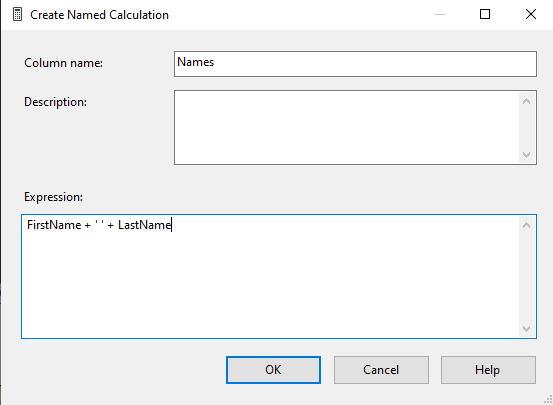
\includegraphics[width=0.6\textwidth]{1a1.png}

  \item W wymiarze SALESPERSON pojawiła się hierarchia Group - CountryRegionCode - Names\\
        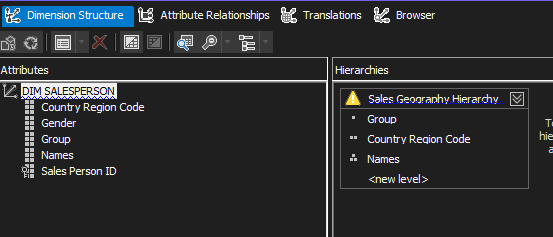
\includegraphics[width=0.6\textwidth]{1a2.png}

  \item W wymiarze CUSTOMER pojawiła się hierarchia Group - CountryRegionCode - Names\\
        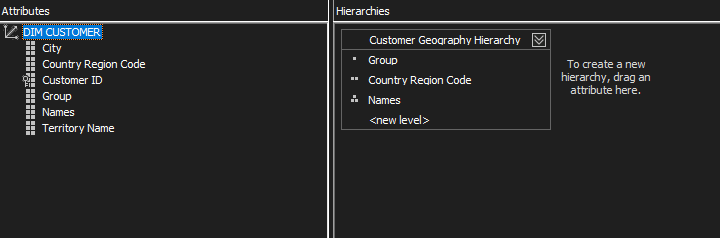
\includegraphics[width=0.6\textwidth]{1a3.png}

  \item W wymiarze PRODUCT pojawiła się hierarchia CategoryName - SubCategoryName - Name\\
        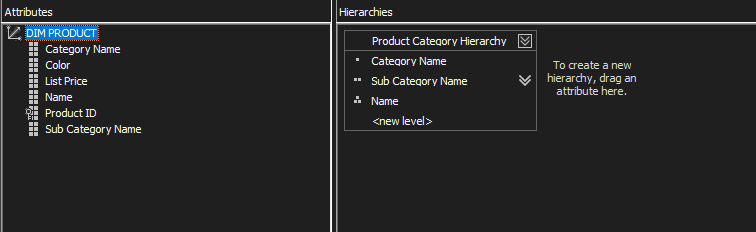
\includegraphics[width=0.6\textwidth]{1a4.png}

  \item W wymiarze TIME pojawiła się hierarchia Rok - Kwartał - Miesiąc - Dzień miesiąca\\
        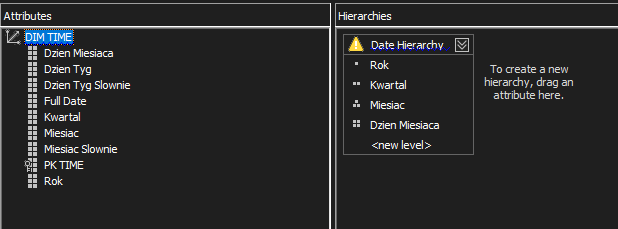
\includegraphics[width=0.6\textwidth]{1a5.png}
\end{enumerate}

\subsection{Podpunkt b}

Dla każdego atrybutu kluczowego wymiaru, którego wartościami są liczby całkowite,
zmodyfikować właściwości (Properties). Zmodyfikować parametr NameColumn, tak
aby nazwy kolejnych elementów wymiaru nie były liczbami. (Przykładowo dla wymiaru dotyczącego Produktu można wykorzystać atrybut Name).

\begin{figure}[H]
  \centering
  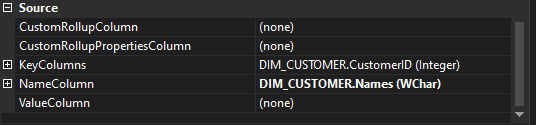
\includegraphics[width=0.6\textwidth]{1b_salesperson.png}
  \caption{Widok Properties dla DIM\_Salesperson}
\end{figure}

\begin{figure}[H]
  \centering
  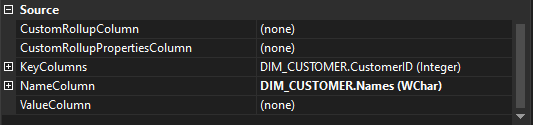
\includegraphics[width=0.6\textwidth]{1b_customer.png}
  \caption{Widok Properties dla DIM\_Customer}
\end{figure}

\begin{figure}[H]
  \centering
  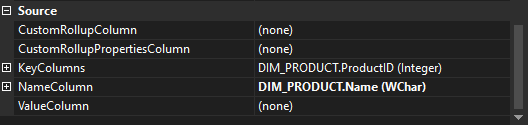
\includegraphics[width=0.6\textwidth]{1b_product.png}
  \caption{Widok Properties dla DIM\_Product}
\end{figure}

\begin{figure}[H]
  \centering
  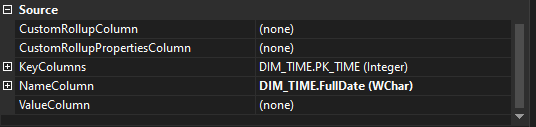
\includegraphics[width=0.6\textwidth]{1b_time.png}
  \caption{Widok Properties dla DIM\_Time}
\end{figure}

\subsection{Podpunkt c}

Utworzyć nowe miary, które będą odzwierciedlać:

\begin{itemize}
  \item Liczbę różnych klientów (aggregatedFunction: distinct count)
  \item Liczbę różnych produktów
  \item Maksymalną wartość rabatu (aggregatedFunction: max)
  \item Maksymalną liczbę zamówionych produktów
  \item Liczbę różnych sprzedawców realizujących zamówienia
\end{itemize}

\begin{figure}[H]
  \centering
  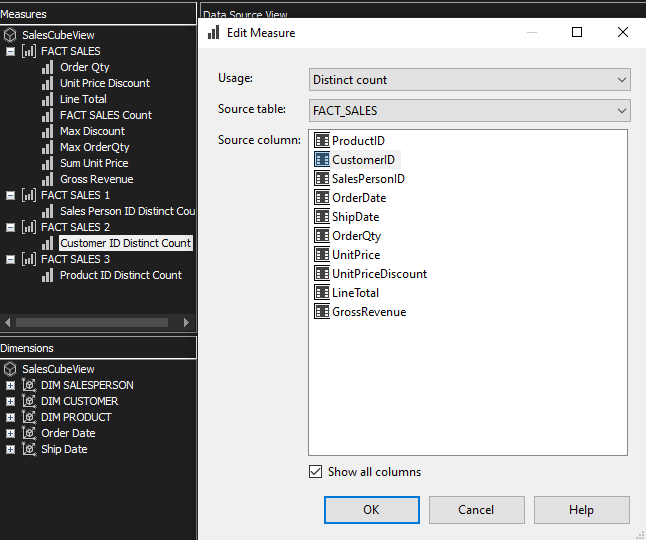
\includegraphics[width=0.6\textwidth]{1c.png}
  \caption{Miara dotycząca liczby różnych klientów}
\end{figure}

\subsection{Podpunkt d}

Wdrożyć i przeprocesować kostkę.

\begin{figure}[H]
  \centering
  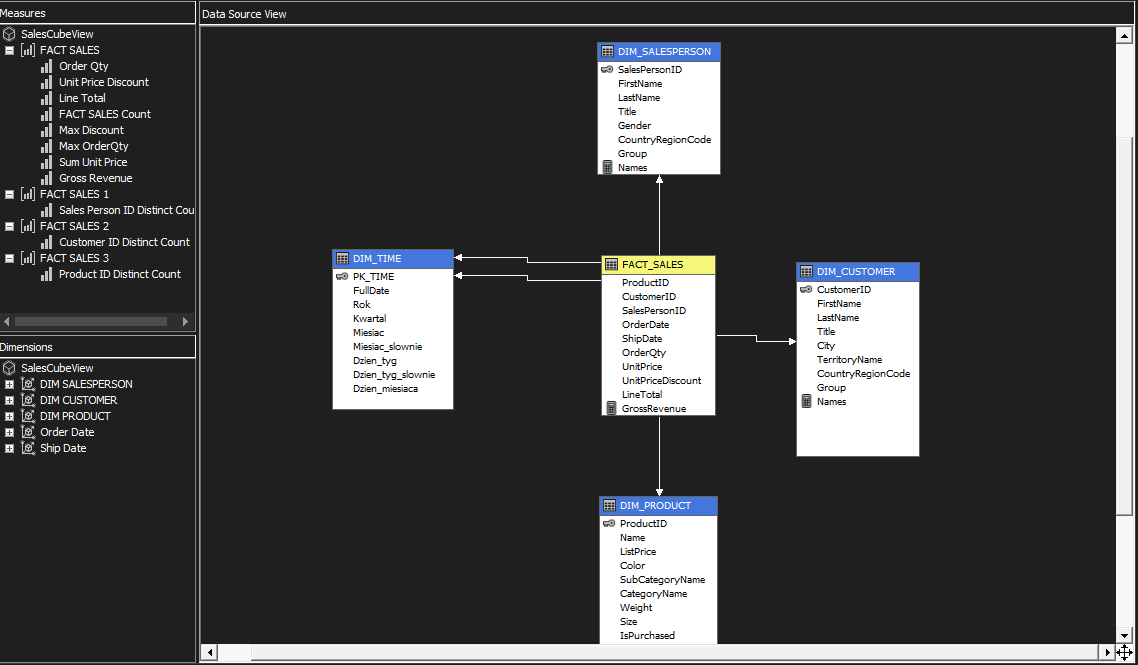
\includegraphics[width=0.6\textwidth]{1d.png}
  \caption{Widok przeprocesowanej kostki}
\end{figure}

\section{Zad. 2. Przegląd danych i tworzenie zestawień}

Przy użyciu zakładki Browser:

\subsection{Podpunkt a}

Sprawdzić, czy dane zapisane w kostce zgadzają się z danymi zapisanymi w tabelach, przeciągając za pomocą myszy:
\begin{itemize}
  \item atrybuty wymiarów w region wierszy
  \item miary w część centralną widoku
\end{itemize}

\begin{figure}[H]
  \centering
  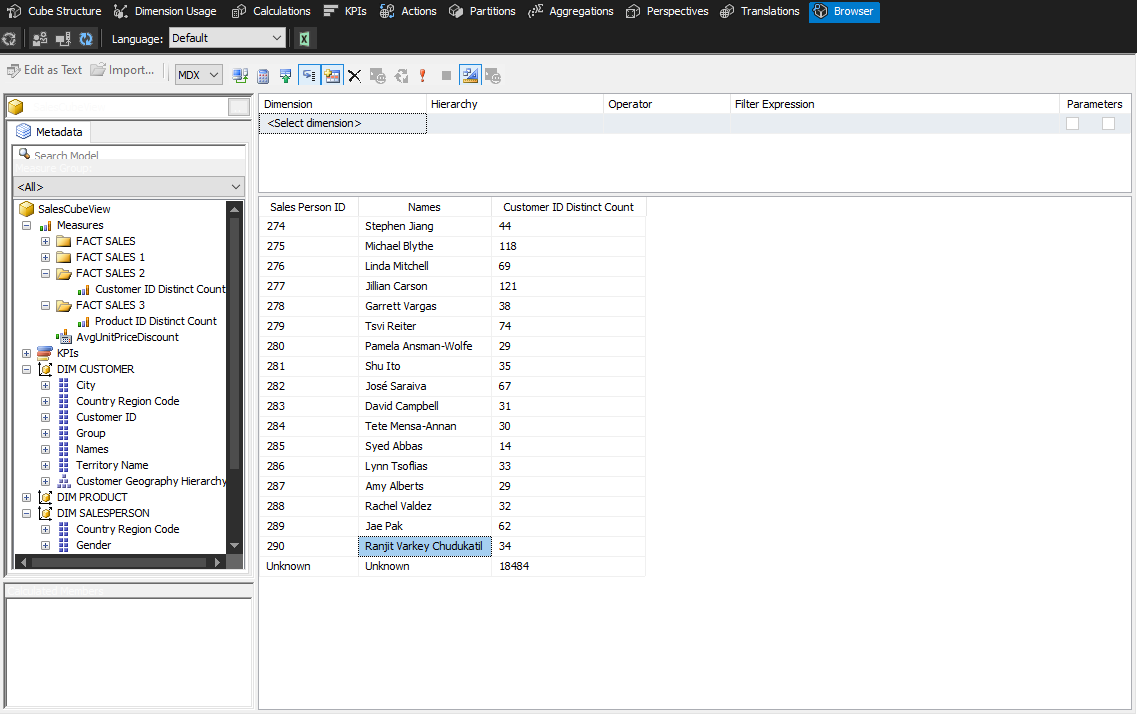
\includegraphics[width=0.6\textwidth]{2a.png}
  \caption{Widok przykładowej kwerendy w Browser}
\end{figure}

\subsection{Podpunkt b}

Przetestować możliwości przeglądarki (Browser) - operator wyboru danych (Operator), wyrażenia filtrujące dane (Filter Expression) itp.

\begin{figure}[H]
  \centering
  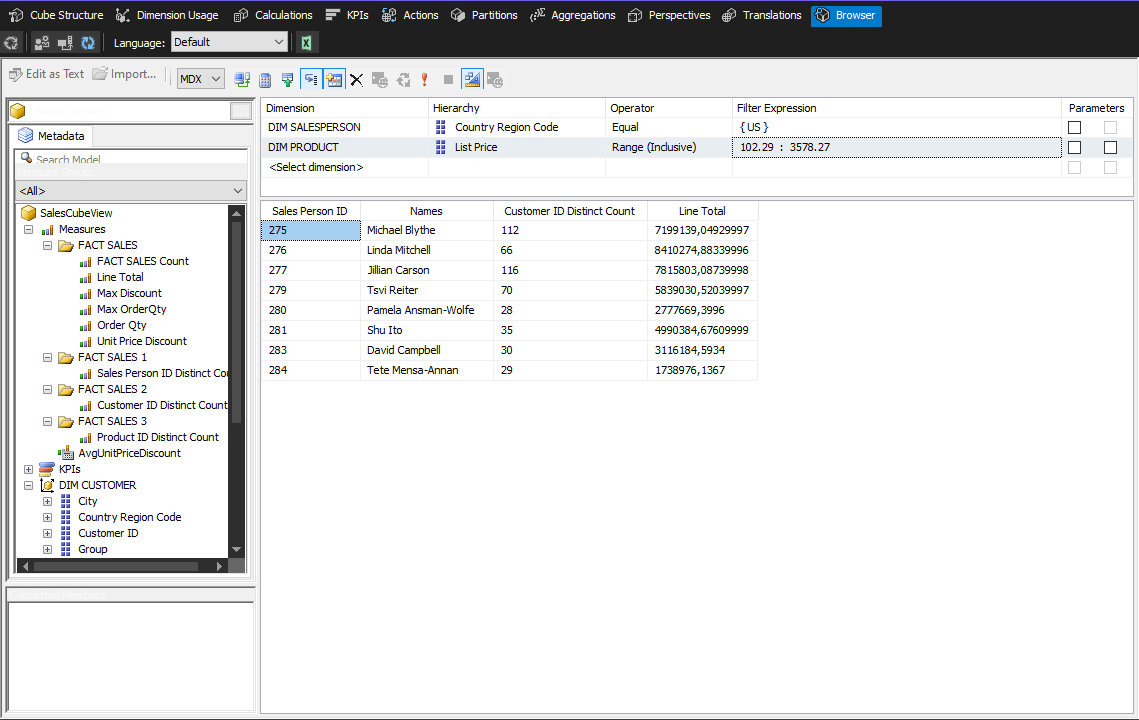
\includegraphics[width=0.6\textwidth]{2b.png}
  \caption{Widok przykładowej kwerendy z dwoma różnymi rodzajami filtrów (Operator i Filter Expression)}
\end{figure}

\subsection{Podpunkt c}

Przygotować przykładowe tabele i wykresy przestawne oraz zinterpretować uzyskane
wyniki (proszę zapisać wnioski!)

\subsubsection{Liczba sprzedanych rowerów w zależności od miesiąca w USA}

\begin{figure}[H]
  \centering
  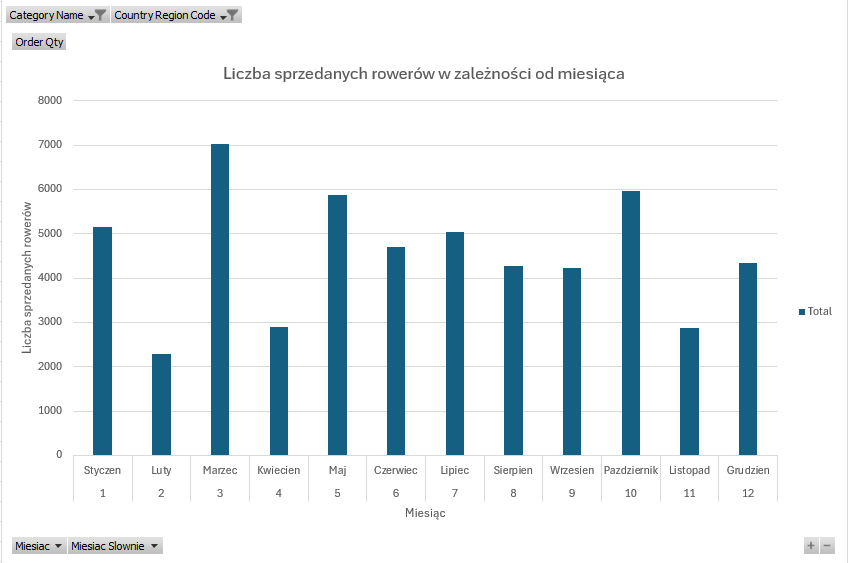
\includegraphics[width=0.6\textwidth]{bike_sales.png}
  \caption{Wykres}
\end{figure}

Na wykres nałożone są 2 filtry - kategoria jest limitowna do rowerów, a kod regionu państwa do USA. Wykres jest posortowane po osi x, czyli związanej z miesiącami, agregując liczbę sprzedanych rowerów dla wszystkich lat naraz.

Generalnie widać trend wzrostu aktywności kupowania w miesiącach letnich. Mimo to, widać również wysokie wartości dla niektórych miesięcy poza sezonem - październik, grudzień, styczeń. Być może np. grudzień jest powiązany ze wzrostem sprzedaży w związku z Bożym Narodzeniem, a październik z potencjalnymi wyprzedażami po sezonie. Marzec osiąga najwiekszą sprzedaż, zaczynając większą sprzedaż sklepu do października. Najmniejsza sprzedaż jest w lutym - raczej popularniejsze są wtedy sporty zimowe.

\subsubsection{Maksymalny rabat udzielony na produkty w latach od kategorii i jego wpływ na średnią ważoną sprzedaży}

\begin{figure}[H]
  \centering
  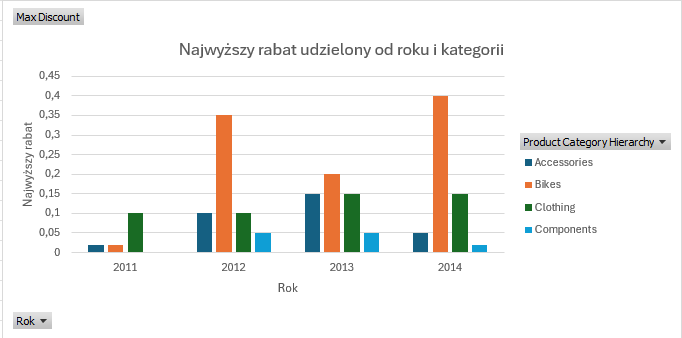
\includegraphics[width=0.6\textwidth]{max_discounts.png}
  \caption{Wykres}
\end{figure}

Na wykresie widać, że najwyższe rabaty udzielane są na rowery. Wartość maksymalnego rabatu w latach 2012-2014 była najwyższa właśnie dla rowerów. Zarówno w 2012, jak i w 2014, ta wartość była bardzo wysoka, około 2 razy wyższa, niż 3. najlepszy wynik (należący do rowerów w 2013 roku). W 2014 roku był udzielony najwyższy rabat ogółem - aż 40\% zniżki dla szczęśliwego klienta.
Ale w 2011, rabaty udzielane dla rowerów były niskie, podobnie jak dla innych kategorii.

Akcesoria - wartość maksymalnego rabatu powoli rosła, z bardzo niskiego poziomu w 2011 do 4. najwyższego ogółem w 2013. Potem w 2014 znowu spadł do niskiego poziomu.

Ubrania - były najbardziej przeceniane w 2011 roku. Były przeceniane na podobnym poziomie w 2012, ale wtedy to rowery je prześcignęły. W 2013 urosły, utrzymując jeden z najwyższych poziomów również w 2014.

Kompnenty - bardzo niskie maksymalne rabaty, zerowe w 2011. W 2012 i 2013 podobne, ale najniższe w zestawieniach, w 2014 znowu spadek do bardzo niskiego poziomu.

Sklep wydaje się mieć dość chaotyczną politykę udzielania rabatów. Należałoby ją lepiej uściślić. Oczywiście, każda kategoria powinna mieć osobną politykę.

Aby przeanalizować wpływ wysokości rabatu na sprzedaż, należy posłużyć się kolejnym wykresem.

\begin{figure}[H]
  \centering
  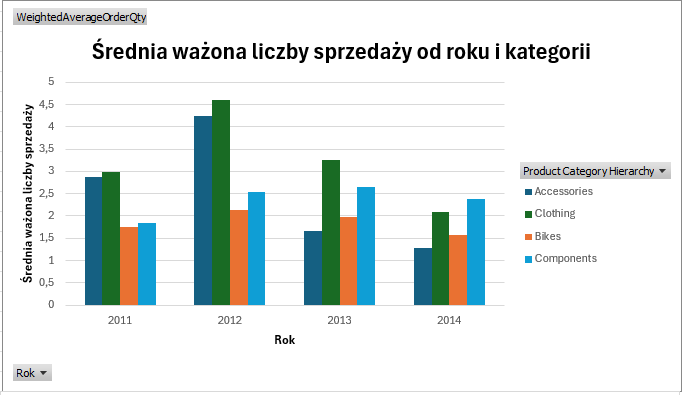
\includegraphics[width=0.6\textwidth]{weighted_sales.png}
  \caption{Wykres}
\end{figure}

Analiza samej średniej ważonej byłaby ciekawa, ale skupiono się na sprawdzeniu relacji między maksymalnym rabatem a średnią ważoną.

Nie widać bezpośredniej relacji między średnią ważoną, a najwyższym rabatem. Często zdarza się, że np. dla rowerów w 2014 roku rabat jest najwyższy, ale średnia ważona sprzedaży jest najniższa od 2012 roku.

Trzeba pamiętać, że każda kategoria może mieć inne statystyki średniej ważonej - naturalne jest to, że klienci kupują akcesoria w większej liczbie niż rowery. Należy więc w sposób ograniczony porównywać różne kategorie między sobą.

Ostatecznie nie stwierdzono zależności między maksymalnym rabatem, a średnią ważoną. Następnym krokiem analizy byłoby sprawdzenie średniego rabatu, gdyż on może zawierać dużo więcej informacji - może w końcu zdarzyć się tak, że maksymalny rabat nie ma silnego powiązania ze średnim rabatem.

\subsubsection{Liczba różnych sprzedanych produktów na sprzedawcę w 3. i 4. kwartale 2013 roku}

\begin{figure}[H]
  \centering
  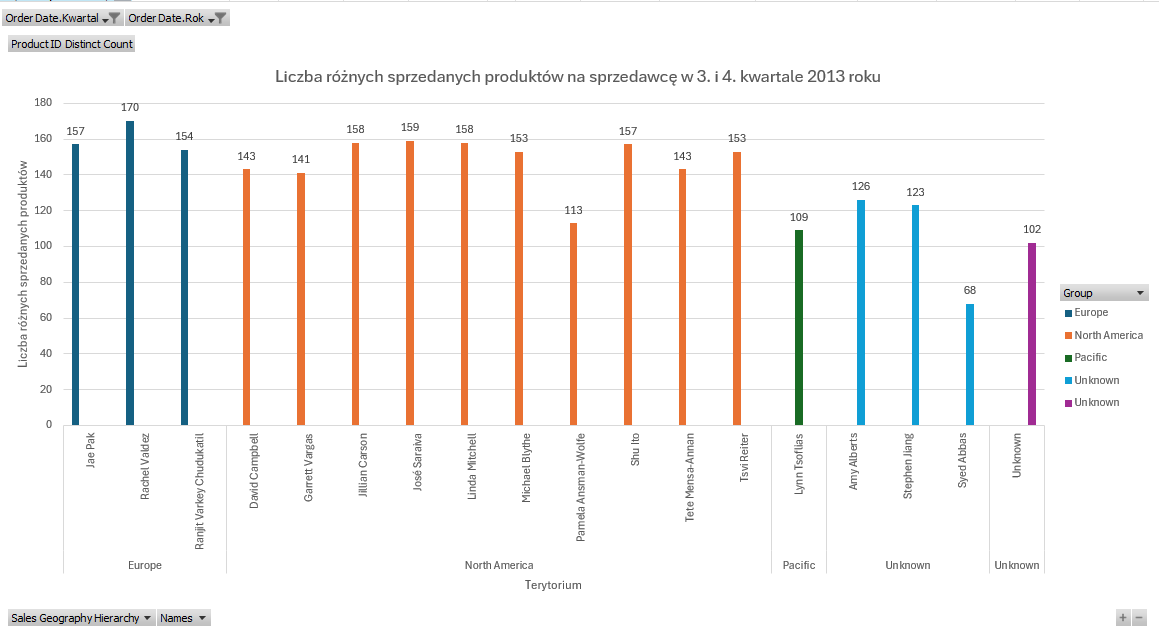
\includegraphics[width=0.6\textwidth]{sales_salesperson.png}
  \caption{Wykres}
\end{figure}

Wykres został arbitralnie ograniczony do 3. i 4. kwartału 2013 roku - mogło by być tak, że menadżer analizuje sytuację w poprzednim roku, czekając na nadejście 3. i 4. kwartału w 2014 roku w bazie danych.

Sprzedawcy utrzymują dość podobny poziom sprzedaży różnych produktów. Bardzo wielu osiąga wysoki poziom ~ 160, zwłaszcza w Europie i w Północnej Ameryce. W rejonie pacyfiku poziom jest niższy, podobny do najniższego poziomu w poprzednich grupach - osiągniętego przez Lindę Mitchell.

Aż 3 sprzedawców nie jest przypisanych do regionu - osiągają oni jedne z niższych wyników sprzedaży różnych produktów.

Wszystkim sprzedawcom osiągającym słabsze wyniki należy przyjrzeć się w celu ewentualnych szkoleń. Jeśli z innych analiz, np. analizy rynku, w którym pracują, ogólnej sprzedaży itd. wyszły również słabe wyniki, byliby to kandydaci do potencjalnych redukcji. Nalezy również koniecznie przypisać sprzedawców bez regionów do regionów - ułatwi to analizę.

\section{Zad. 3. Miary kalkulowane}

W zakładce Calculations dodać dwie miary kalkulowane (ang. calculated members):\begin{itemize}
  \item średnią liczbę zamówionych towarów na zamówienie
  \item średnią ważoną liczbę towarów na zamówienie. Jako wagę należy wybrać cenę danego produktu.
\end{itemize}
Wskazówka: w celu utworzenia wyżej wymienionej średniej ważonej można posłużyć się nową
kolumną zdefiniowaną w widoku źródła danych (lub w tabeli). Kolumna ta powinna definiować
miarę pomocniczą, która pozwoli uzyskać fragment wyrażenia odpowiadającego średniej
ważonej.

\begin{figure}[H]
  \centering
  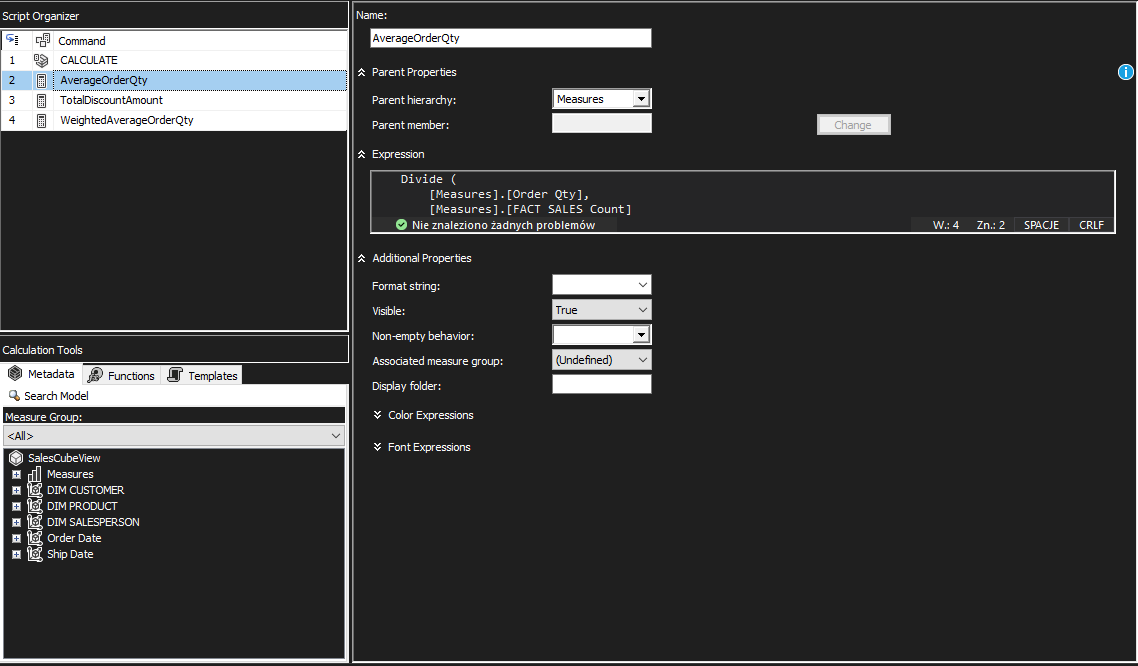
\includegraphics[width=0.6\textwidth]{3_calculations_1.png}
  \caption{Sposób obliczania miary ze zwykłą średnią}
\end{figure}

Do obliczenia średniej ważonej należało dodać miarę obliczającą sumę ceny jednostkowej i drugą miarę, będącą iloczynem ceny jednostkowej i liczby zamówionego produktu (LineTotal prawie to spełniał, ale miał w sobie czasem zniżkę).

\begin{figure}[H]
  \centering
  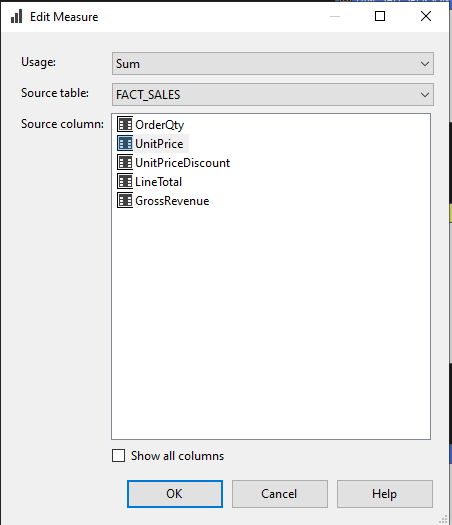
\includegraphics[width=0.6\textwidth]{3_sum_unit_price.png}
  \caption{Sposób obliczania miary z sumą ceny jednostkowej}
\end{figure}

\begin{figure}[H]
  \centering
  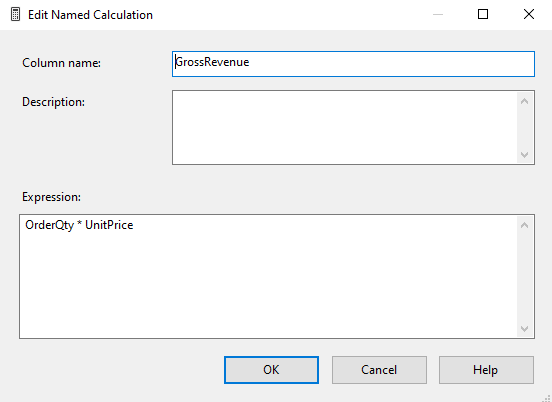
\includegraphics[width=0.6\textwidth]{3_gross_revenue.png}
  \caption{Sposób obliczania miary zysku brutto}
\end{figure}

\begin{figure}[H]
  \centering
  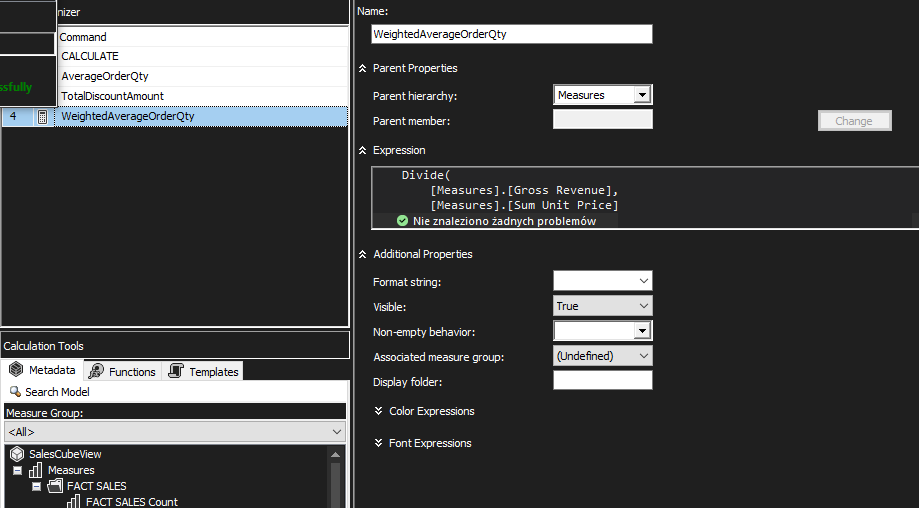
\includegraphics[width=0.6\textwidth]{3_calculations_2.png}
  \caption{Sposób obliczania miary średniej ważonej}
\end{figure}

\begin{figure}[H]
  \centering
  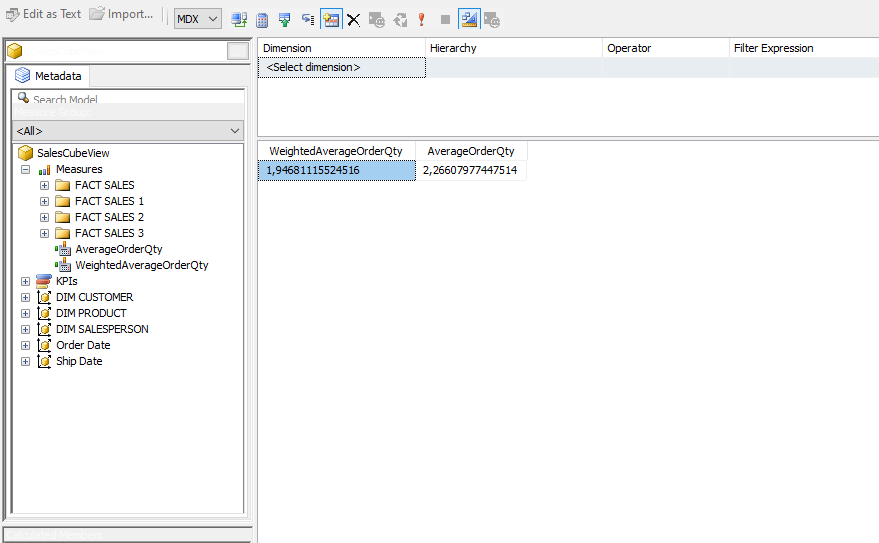
\includegraphics[width=0.6\textwidth]{3_result.png}
  \caption{Wynik średnich dla całego zbioru danych}
\end{figure}

Średnia ważona wynosi około 1.96, a zwykła średnia około 2.27. Średnia ważona jest niższa prawdopodobnie dlatego, że klienci kupują droższe produkty w statystycznie mniejszej liczbie, niż tańsze.

\section{Zad. 4. Partycje}

Podzielić zawartość kostki na partycje (zakładka Partitions). Każda partycja powinna
odzwierciedlać jeden rok. Istnieją dwa podstawowe sposoby podziału partycjonowania kostek:
\begin{itemize}
  \item dane do zasilania poszczególnych partycji znajdują się w osobnych tabelach
  \item dane do zasilania poszczególnych partycji znajdują się w tej samej tabeli, zaś każda z partycji ma przypisanie zapytanie SQL, którego wynik służy do jej zasilenia.
\end{itemize}
Proszę przygotować partycje na dwa sposoby i znaleźć uzasadnienie dla każdej opcji.

\subsection{Sposób pierwszy}

Ta metoda wymagała utworzenia w bazie SQL Server osobnych tabel dla każdego roku (np. `FACT\_SALES\_2011`, `FACT\_SALES\_2012`, itd.)
o strukturze identycznej jak oryginalna tabela faktów, a następnie wypełnienia ich danymi z odpowiednich lat.

\begin{lstlisting}[caption={Tworzenie i wypełnianie tabeli DIM\_TIME.}]
CREATE TABLE Kubs.FACT_SALES_2011 (
  ProductID INT FOREIGN KEY REFERENCES Kubs.DIM_PRODUCT(ProductID),
    CustomerID INT FOREIGN KEY REFERENCES Kubs.DIM_CUSTOMER(CustomerID),
    SalesPersonID INT FOREIGN KEY REFERENCES Kubs.DIM_SALESPERSON(SalesPersonID),
    OrderDate INT NOT NULL,
    ShipDate INT NULL,
    OrderQty SMALLINT NOT NULL,
    UnitPrice MONEY NOT NULL,
    UnitPriceDiscount DECIMAL(8, 4) NOT NULL,
    LineTotal DECIMAL(19, 4) NOT NULL
);

CREATE TABLE Kubs.FACT_SALES_2012 (
  ProductID INT FOREIGN KEY REFERENCES Kubs.DIM_PRODUCT(ProductID),
    CustomerID INT FOREIGN KEY REFERENCES Kubs.DIM_CUSTOMER(CustomerID),
    SalesPersonID INT FOREIGN KEY REFERENCES Kubs.DIM_SALESPERSON(SalesPersonID),
    OrderDate INT NOT NULL,
    ShipDate INT NULL,
    OrderQty SMALLINT NOT NULL,
    UnitPrice MONEY NOT NULL,
    UnitPriceDiscount DECIMAL(8, 4) NOT NULL,
    LineTotal DECIMAL(19, 4) NOT NULL
);

CREATE TABLE Kubs.FACT_SALES_2013 (
  ProductID INT FOREIGN KEY REFERENCES Kubs.DIM_PRODUCT(ProductID),
    CustomerID INT FOREIGN KEY REFERENCES Kubs.DIM_CUSTOMER(CustomerID),
    SalesPersonID INT FOREIGN KEY REFERENCES Kubs.DIM_SALESPERSON(SalesPersonID),
    OrderDate INT NOT NULL,
    ShipDate INT NULL,
    OrderQty SMALLINT NOT NULL,
    UnitPrice MONEY NOT NULL,
    UnitPriceDiscount DECIMAL(8, 4) NOT NULL,
    LineTotal DECIMAL(19, 4) NOT NULL
);

CREATE TABLE Kubs.FACT_SALES_2014 (
  ProductID INT FOREIGN KEY REFERENCES Kubs.DIM_PRODUCT(ProductID),
    CustomerID INT FOREIGN KEY REFERENCES Kubs.DIM_CUSTOMER(CustomerID),
    SalesPersonID INT FOREIGN KEY REFERENCES Kubs.DIM_SALESPERSON(SalesPersonID),
    OrderDate INT NOT NULL,
    ShipDate INT NULL,
    OrderQty SMALLINT NOT NULL,
    UnitPrice MONEY NOT NULL,
    UnitPriceDiscount DECIMAL(8, 4) NOT NULL,
    LineTotal DECIMAL(19, 4) NOT NULL
);

with Sales1 AS (
  SELECT 
    Kubs.FACT_SALES.ProductID,
    Kubs.FACT_SALES.CustomerID,
    Kubs.FACT_SALES.SalesPersonID,
    Kubs.FACT_SALES.OrderDate,
    Kubs.FACT_SALES.ShipDate,
    Kubs.FACT_SALES.OrderQty,
    Kubs.FACT_SALES.UnitPrice,
    Kubs.FACT_SALES.UnitPriceDiscount,
    Kubs.FACT_SALES.LineTotal
  FROM Kubs.FACT_SALES
  WHERE OrderDate >= 20110101 AND OrderDate < 20120000
)
INSERT INTO Kubs.FACT_SALES_2011

with Sales2 AS (
  SELECT 
    Kubs.FACT_SALES.ProductID,
    Kubs.FACT_SALES.CustomerID,
    Kubs.FACT_SALES.SalesPersonID,
    Kubs.FACT_SALES.OrderDate,
    Kubs.FACT_SALES.ShipDate,
    Kubs.FACT_SALES.OrderQty,
    Kubs.FACT_SALES.UnitPrice,
    Kubs.FACT_SALES.UnitPriceDiscount,
    Kubs.FACT_SALES.LineTotal
  FROM Kubs.FACT_SALES
  WHERE OrderDate >= 20120101 AND OrderDate < 20130000
)
INSERT INTO Kubs.FACT_SALES_2012

with Sales3 AS (
  SELECT 
    Kubs.FACT_SALES.ProductID,
    Kubs.FACT_SALES.CustomerID,
    Kubs.FACT_SALES.SalesPersonID,
    Kubs.FACT_SALES.OrderDate,
    Kubs.FACT_SALES.ShipDate,
    Kubs.FACT_SALES.OrderQty,
    Kubs.FACT_SALES.UnitPrice,
    Kubs.FACT_SALES.UnitPriceDiscount,
    Kubs.FACT_SALES.LineTotal
  FROM Kubs.FACT_SALES
  WHERE OrderDate >= 20130101 AND OrderDate < 20140000
)
INSERT INTO Kubs.FACT_SALES_2013

with Sales4 AS (
  SELECT 
    Kubs.FACT_SALES.ProductID,
    Kubs.FACT_SALES.CustomerID,
    Kubs.FACT_SALES.SalesPersonID,
    Kubs.FACT_SALES.OrderDate,
    Kubs.FACT_SALES.ShipDate,
    Kubs.FACT_SALES.OrderQty,
    Kubs.FACT_SALES.UnitPrice,
    Kubs.FACT_SALES.UnitPriceDiscount,
    Kubs.FACT_SALES.LineTotal
  FROM Kubs.FACT_SALES
  WHERE OrderDate >= 20140101
)
INSERT INTO Kubs.FACT_SALES_2014
\end{lstlisting}

Następnie należało dodać każdą z tabel do projektu, a potem do partycji w kostce.

\begin{figure}[H]
  \centering
  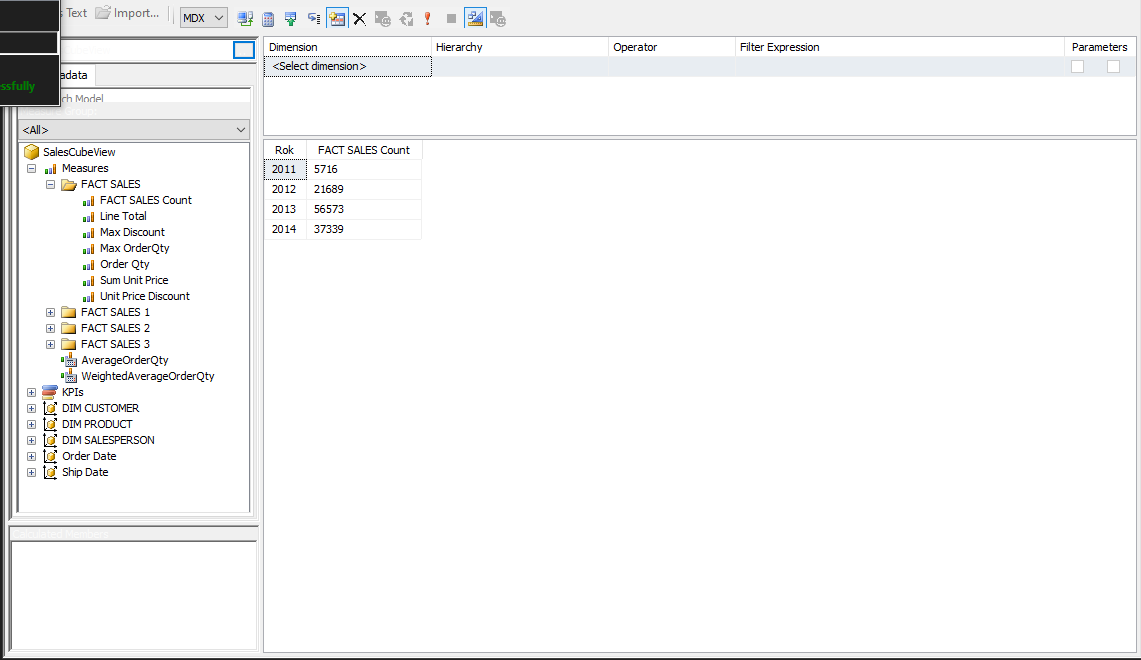
\includegraphics[width=0.6\textwidth]{4a.png}
  \caption{Dodane partycje}
\end{figure}

\begin{figure}[H]
  \centering
  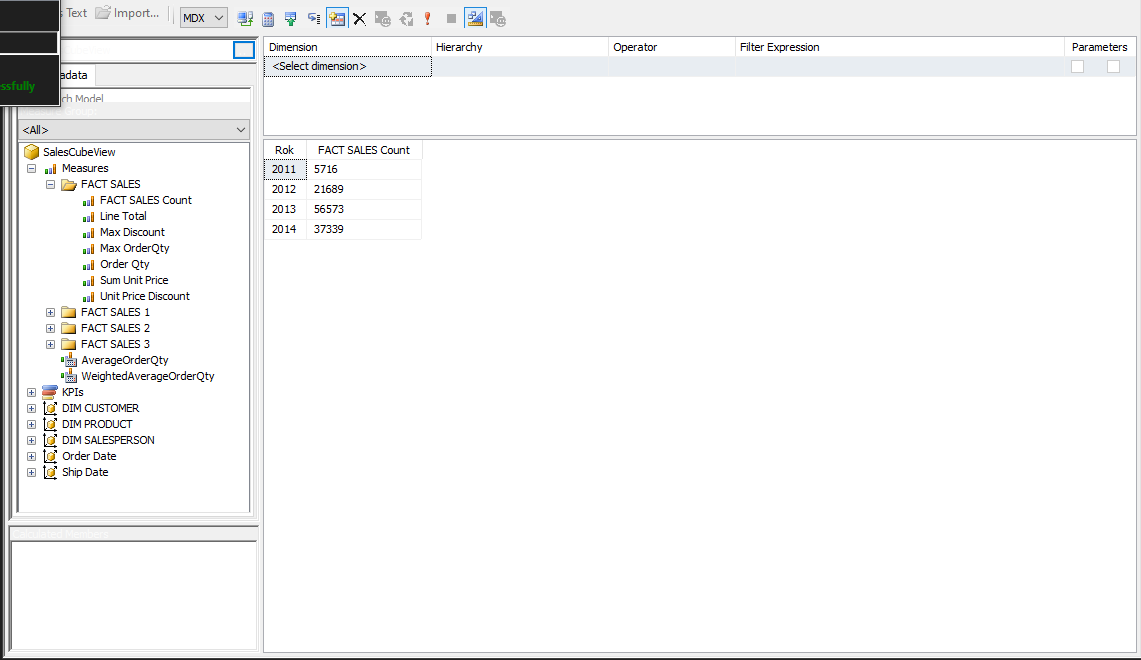
\includegraphics[width=0.6\textwidth]{4a_result.png}
  \caption{Wynik}
\end{figure}

\textit{Uzasadnienie:} Lepsza izolacja danych, potencjalnie szybsze przetwarzanie partycji (odczyt z mniejszych tabel), zgodność z procesami ETL ładującymi dane rocznie, większa możliwość automatyzacji procesu, zwłaszcza dla zmieniających się danych - tak jak tutaj, dla lat.

\subsection{Sposób drugi}

W tej metodzie wszystkie dane pozostają w oryginalnej tabeli `FACT\_SALES`. Partycje tworzone są przez zdefiniowanie
zapytania SQL (query binding) dla każdej z nich, które wybiera dane tylko dla konkretnego roku za pomocą klauzuli `WHERE`

\begin{figure}[H]
  \centering
  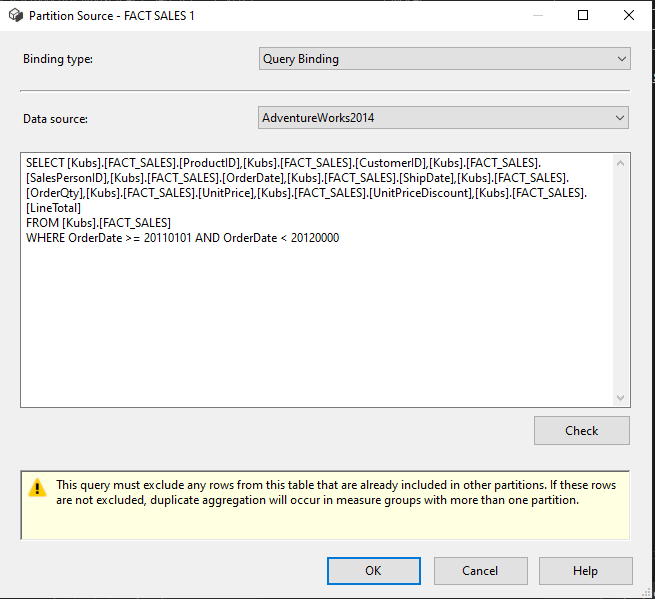
\includegraphics[width=0.6\textwidth]{4b_source.png}
  \caption{Zmieniony kod SQL w partycji - dodana klauzula WHERE ograniczająca daty}
\end{figure}

\begin{figure}[H]
  \centering
  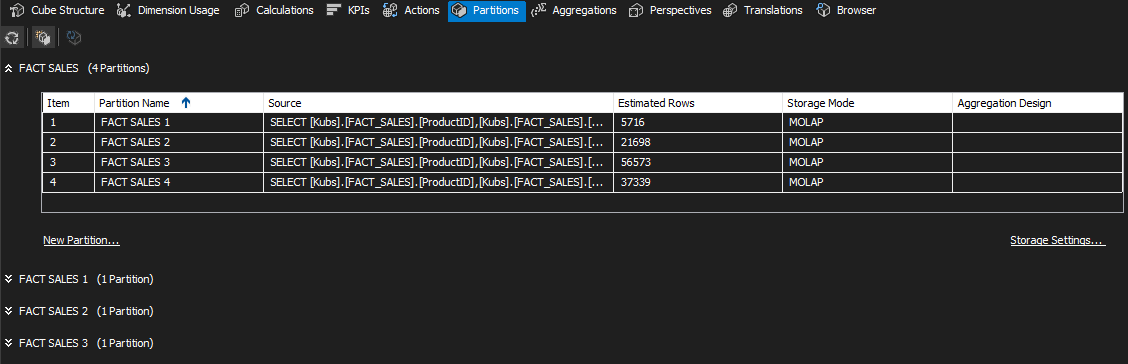
\includegraphics[width=0.6\textwidth]{4b.png}
  \caption{Dodane partycje}
\end{figure}

\begin{figure}[H]
  \centering
  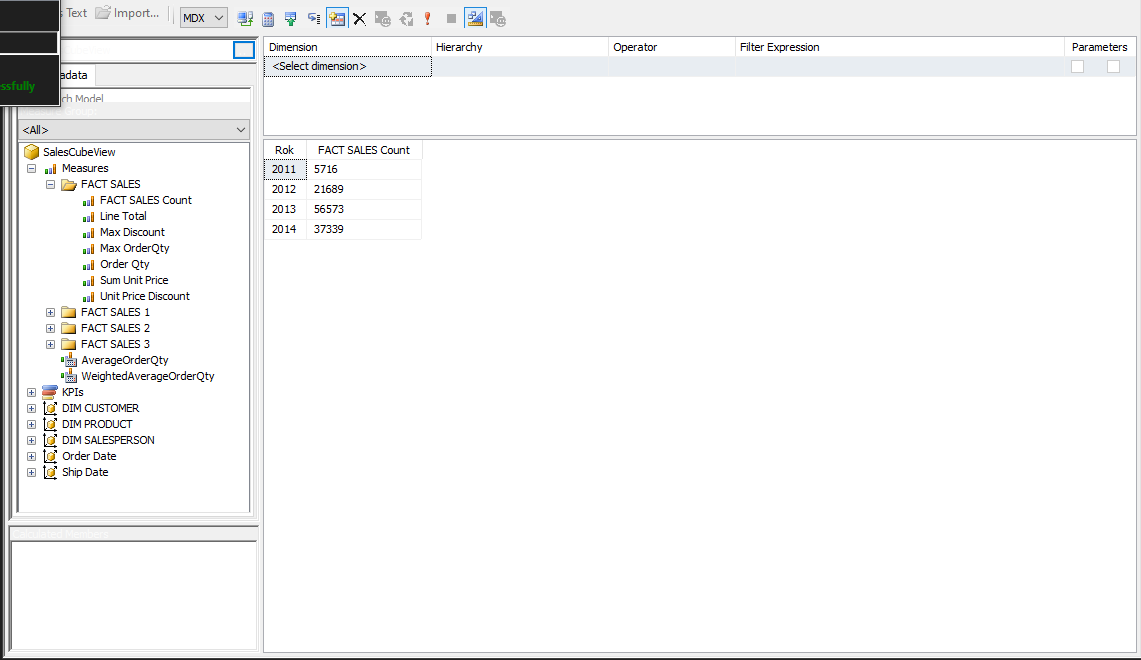
\includegraphics[width=0.6\textwidth]{4a_result.png}
  \caption{Wynik}
\end{figure}

\textit{Uzasadnienie:} Brak konieczności tworzenia dodatkowych tabel w bazie SQL, prostsze zarządzanie bazą danych, łatwiejsza zmiana kryteriów partycjonowania (modyfikacja zapytań).

\section{Zad. 5. * Definiowanie KPI}

\subsection{Prosty wskaźnik KPI}

Przygotować wskaźnik KPI (zakładka \textit{KPI}), która umożliwi podział klientów na dobrych i lepszych w zależności od liczby sztuk zamówionych produktów.

Tworząc nowy wskaźnik należy podać jego nazwę, wybrać (przeciągnąć) miarę, na podstawie której będzie dokonany podział zbioru, wybrać odpowiedni status (np. \textit{Shapes}) i podać warunek:
\[
  \text{iif}([\text{Measures}].[OrderQty] < \eta, -1 \text{ /*czerwony*/}, 1 \text{ /*zielony*/})
\]

Należy uzasadnić wybór wartości progowej $\eta$.

Po przeprocesowaniu kostki, należy zobrazować działanie wskaźnika dla wybranych atrybutów w raporcie w Excelu.

Postanowiono przyjąć KPI dzielące klientów na 2 grupy - około top 20\% "elitarnych" klientów i całą resztę.

\begin{lstlisting}[caption={Kwerenda znajdująca dane do wyliczenia KPI}]
SELECT TOP 20 PERCENT OrderQty
FROM Kubs.FACT_SALES
ORDER BY OrderQty DESC;
\end{lstlisting}

Po krótkiej analizie wyników okazało się, że wartość progową $\eta$ można wyznaczyć jako 4. Tak więc kliencie, którzy kupili co najmniej 4 przedmioty, są elitarni.

Wybór wartości granicznej równej 20\% wynika z konceptu \textit{„krzywej wieloryba”} (ang. \textit{whale curve}), gdzie:
\begin{itemize}
  \item Top 20\% klientów generuje ponad 100\% zysku,
  \item Środkowe 60\% klientów przynosi niewielki zysk lub bilansuje się,
  \item Najsłabsze 20\% klientów generuje straty, przez co łączny zysk netto wraca do poziomu poniżej 100\%.
\end{itemize}

Koncepcja ta pomaga zrozumieć, że niewielka część klientów odpowiada za większość rentowności firmy, co uzasadnia przyjęcie progu 20\% w konstrukcji KPI. \cite{whale_curve}

\begin{figure}[H]
  \centering
  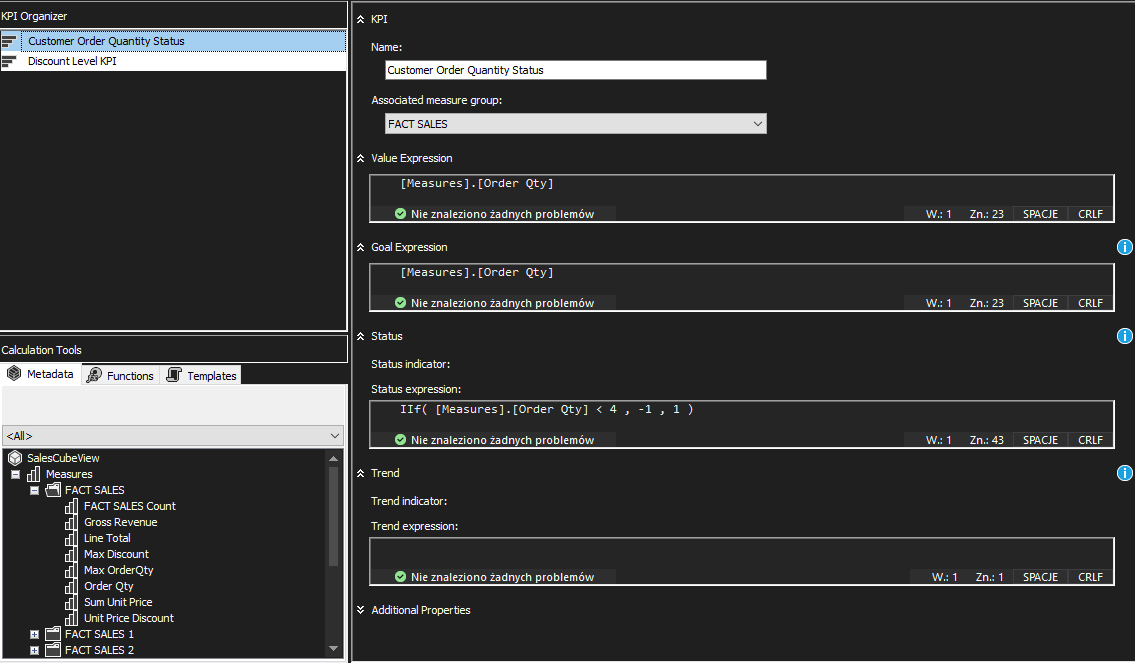
\includegraphics[width=0.6\textwidth]{5a.png}
  \caption{Sposób obliczenia KPI}
\end{figure}

\begin{figure}[H]
  \centering
  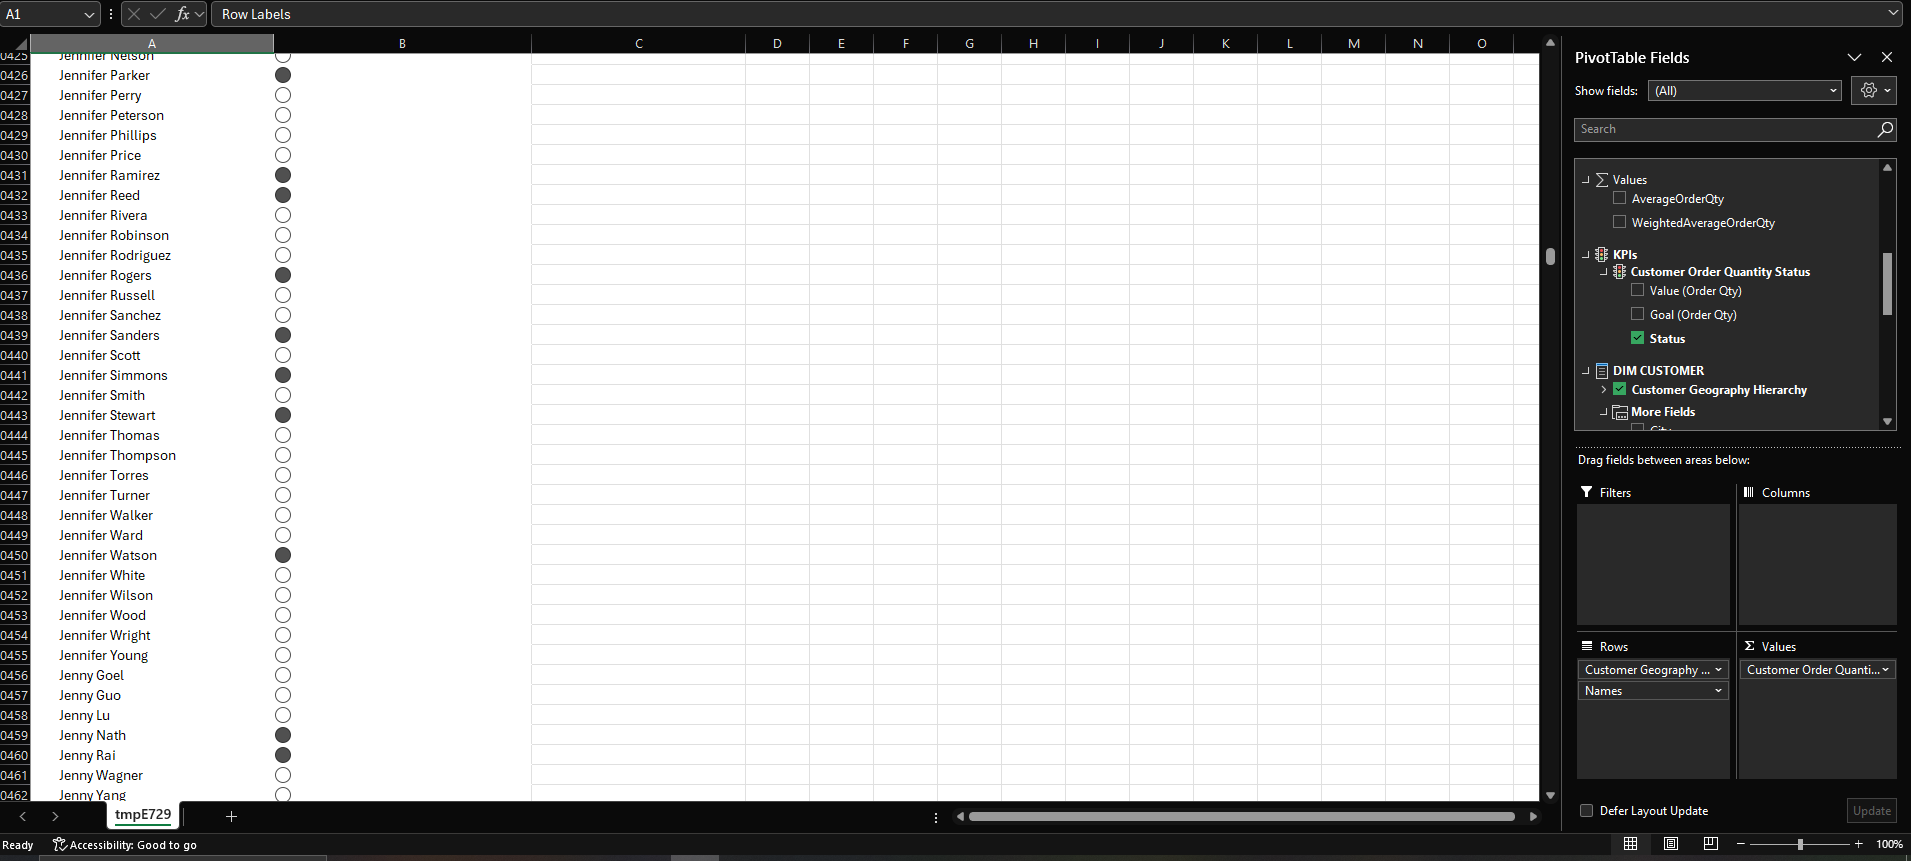
\includegraphics[width=0.6\textwidth]{5a_analysis.png}
  \caption{Tabela przestawna z widokiem na wartości KPI}
\end{figure}

\subsection{KPI na podstawie kalkulowanej miary}

Zaproponować własną miarę w zakładce \textit{Calculation $\rightarrow$ New Calculated Member},
(np. zysk z uwzględnieniem rabatu i frachtu), na podstawie której zostanie zdefiniowany odpowiedni wskaźnik KPI. Należy przeanalizować status opracowanego wskaźnika oraz jego trend. Wynik należy zaprezentować w wybranym kontekście.

Zdefiniowano własną miarę kalkulowaną `Total Discount Amount` (Całkowita Wartość Rabatu) jako różnicę między przychodem brutto (wymagało użycia dodanej wcześniej miary `Gross Revenue`) a przychodem netto (`Line Total`).

Na podstawie tej miary stworzono `Discount Level KPI`, który ocenia poziom rabatu względem przychodu brutto (cel: <= .5\%, źle: > .8\%) oraz pokazuje trend porównując wartość rabatu do roku poprzedniego.

\begin{figure}[H]
  \centering
  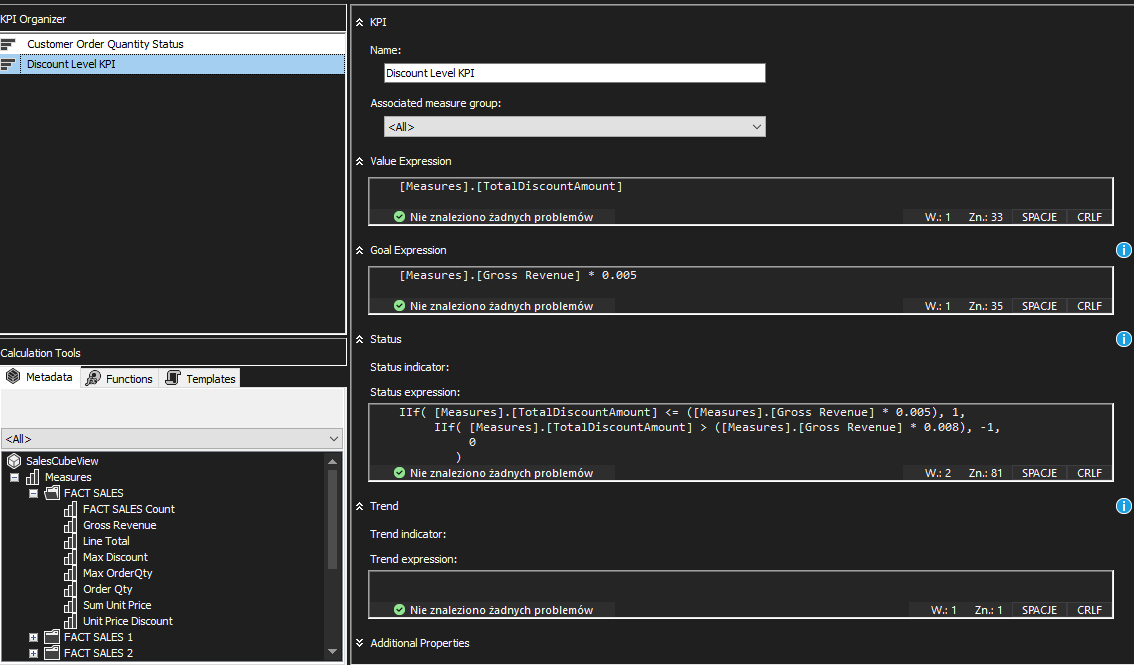
\includegraphics[width=0.6\textwidth]{5b.png}
  \caption{Sposób obliczenia KPI}
\end{figure}

\begin{figure}[H]
  \centering
  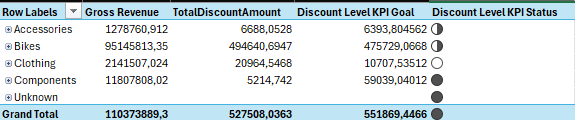
\includegraphics[width=0.6\textwidth]{5b_analysis.png}
  \caption{Tabela przestawna z widokiem na wartości KPI}
\end{figure}

\begin{figure}[H]
  \centering
  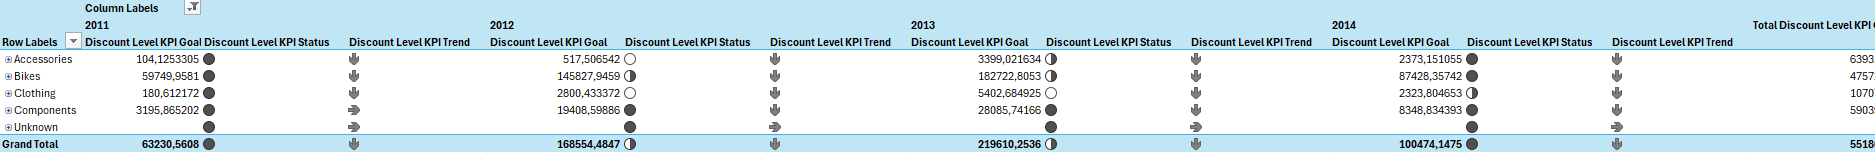
\includegraphics[width=0.6\textwidth]{5b_analysis_2.png}
  \caption{Tabela przestawna z widokiem na wartości KPI z trendami}
\end{figure}

\section{Wnioski}

Realizacja laboratorium pozwoliła na pogłębienie wiedzy na temat zaawansowanych funkcji SSAS.

Modyfikacja wymiarów i tworzenie hierarchii znacząco poprawia czytelność i możliwości analizy danych w kostce OLAP, umożliwiając drążenie danych.

Miary kalkulowane pozwalają na definiowanie bardziej złożonych wskaźników biznesowych bezpośrednio w kostce przy użyciu MDX, bez konieczności modyfikacji źródła danych.

Różnica między średnią arytmetyczną a ważoną może być znacząca w zależności od kontekstu biznesowego. W tym biznesie raczej większe znaczenie będzie miała dobra średnia ważone, gdyż przekazuje ona więcej informacji o znaczeniu biznesowym.

Partycjonowanie tabel faktów jest kluczową techniką optymalizacyjną, szczególnie dla dużych hurtowni danych, przyspieszając przetwarzanie i potencjalnie zapytania. Wybór metody partycjonowania (osobne tabele vs zapytania) zależy od specyfiki systemu źródłowego i procesów ETL.

Definiowanie KPI umożliwia szybką wizualną ocenę kluczowych wskaźników biznesowych oraz ich trendów, co jest niezwykle przydatne w raportowaniu i analizie menedżerskiej.
Z drugiej strony, trzeba uważać na złe KPI - stworzona w drugim podpunkcie KPI może wprowadzić w błąd trendem ujemnym. W tym przypadku po głębszej analizie okazuje się, że ponieważ zyski sklepu i jego popularność rosną, to zwiększyła się liczba zniżek. Można by ulepszyć KPI, by trend brał pod uwagę zmiany w sprzedaży ogólnie - aktualnie tego nie robi.

\printbibliography

\end{document}